\documentclass[11pt]{article}
\usepackage{amsmath}
\usepackage{amssymb}
\usepackage{graphicx}
\usepackage{tabularx}
\usepackage{fancyhdr}
\usepackage{lastpage}

% Page layout
\usepackage[top=1in, bottom=1in, left=1in, right=1in]{geometry}

% Header and footer
\pagestyle{fancy}
\fancyhf{}
\rfoot{Page \thepage}
\renewcommand{\headrulewidth}{0pt}

% Modified Question command with left-aligned number
\newcommand{\questiona}[2]{
    \noindent\textbf{Q#2.} #1 \hfill \textbf{[1 Mark]}
}

\newcommand{\questionb}[2]{
    \noindent\textbf{Q#2.} #1 \hfill \textbf{[2 Marks]}
}

\begin{document}

% Title section with horizontal line
\begin{center}
    \Large\textbf{GATE 2017 - Civil Engineering (CE)} \\
    \large\textbf{General Aptitude and Technical Questions} \\
    \rule{\textwidth}{0.5pt} % Horizontal line below heading
\end{center}

\vspace{0.5cm}

% General Aptitude Section
\section*{General Aptitude}

% General Aptitude Section
\section*{General Aptitude}

\questiona{The event would have been successful if you \_\_\_\_\_ able to come.}{1}
\begin{enumerate}
    \item[(A)] are  
    \item[(B)] had been  
    \item[(C)] have been  
    \item[(D)] would have been  
\end{enumerate}

\vspace{0.5cm}

\questiona{There was no doubt that their work was thorough.

Which of the words below is closest in meaning to the underlined word above?}{2}
\begin{enumerate}
    \item[(A)] pretty  
    \item[(B)] complete  
    \item[(C)] sloppy  
    \item[(D)] haphazard  
\end{enumerate}

\vspace{0.5cm}

\questiona{Four cards lie on a table. Each card has a number printed on one side and a colour on the other. The faces visible on the cards are 2, 3, red, and blue.

Proposition: If a card has an even value on one side, then its opposite face is red.

The cards which MUST be turned over to verify the above proposition are}{3}
\begin{enumerate}
    \item[(A)] 2, red  
    \item[(B)] 2, 3, red  
    \item[(C)] 2, blue  
    \item[(D)] 2, red, blue  
\end{enumerate}

\vspace{0.5cm}

\questiona{What is the value of \( x \) when \( 81 \times \left( \frac{16}{25} \right)^{x+2} \div \left( \frac{3}{5} \right)^{2x+4} = 144 \)?}{4}
\begin{enumerate}
    \item[(A)] 1  
    \item[(B)] -1  
    \item[(C)] -2  
    \item[(D)] Cannot be determined  
\end{enumerate}

\vspace{0.5cm}

\questiona{Two dice are thrown simultaneously. The probability that the product of the numbers appearing on the top faces of the dice is a perfect square is}{5}
\begin{enumerate}
    \item[(A)] 1/9  
    \item[(B)] 2/9  
    \item[(C)] 1/3  
    \item[(D)] 4/9  
\end{enumerate}

\vspace{0.5cm}

\questionb{Bhaichung was observing the pattern of people entering and leaving a car service centre. There was a single window where customers were being served. He saw that people inevitably came out of the centre in the order that they went in. However, the time they spent inside seemed to vary a lot: some people came out in a matter of minutes while for others it took much longer.

From this, what can one conclude?}{6}
\begin{enumerate}
    \item[(A)] The centre operates on a first-come-first-served basis, but with variable service times, depending on specific customer needs.
    \item[(B)] Customers were served in an arbitrary order, since they took varying amounts of time for service completion in the centre.
    \item[(C)] Since some people came out within a few minutes of entering the centre, the system is likely to operate on a last-come-first-served basis.
    \item[(D)] Entering the centre early ensured that one would have shorter service times and most people attempted to do this.
\end{enumerate}

\vspace{0.5cm}

\questionb{A map shows the elevations of Darjeeling, Gangtok, Kalimpong, Pelling, and Siliguri.
Kalimpong is at a lower elevation than Gangtok. Pelling is at a lower elevation than Gangtok.
Pelling is at a higher elevation than Siliguri. Darjeeling is at a higher elevation than Gangtok.

Which of the following statements can be inferred from the paragraph above?
\begin{enumerate}
\item [i.] Pelling is at a higher elevation than Kalimpong
\item [ii.] Kalimpong is at a lower elevation than Darjeeling
\item [iii.] Kalimpong is at a higher elevation than Siliguri
\item [iv.] Siliguri is at a lower elevation than Gangtok
\end{enumerate}}{7}
\begin{enumerate}
    \item[(A)] Only ii
    \item[(B)] Only ii and iii
    \item[(C)] Only ii and iv
    \item[(D)] Only iii and iv
\end{enumerate}

\vspace{0.5cm}

\questionb{P, Q, R, S, T and U are seated around a circular table. R is seated two places to the right of Q. P is seated three places to the left of R. S is seated opposite U. If P and U now switch seats, which of the following must necessarily be true?}{8}
\begin{enumerate}
    \item[(A)] P is immediately to the right of R
    \item[(B)] T is immediately to the left of P
    \item[(C)] T is immediately to the left of P or P is immediately to the right of Q
    \item[(D)] U is immediately to the right of R or P is immediately to the left of T
\end{enumerate}

\vspace{0.5cm}

\questionb{Budhan covers a distance of 19 km in 2 hours by cycling one fourth of the time and walking the rest. The next day he cycles (at the same speed as before) for half the time and walks the rest (at the same speed as before) and covers 26 km in 2 hours. The speed in km/h at which Budhan walks is}{9}
\begin{enumerate}
    \item[(A)] 1
    \item[(B)] 4
    \item[(C)] 5
    \item[(D)] 6
\end{enumerate}

\vspace{0.5cm}

\questionb{The points in the graph below represent the halts of a lift for durations of 1 minute, over a period of 1 hour.

\begin{center}
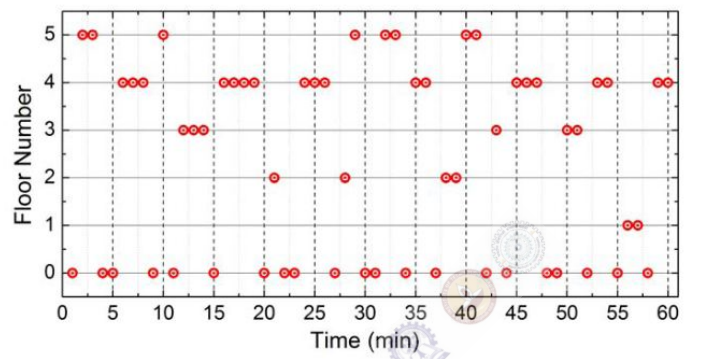
\includegraphics[width=0.5\textwidth]{figures/10.png}
\end{center}

Which of the following statements are correct?

i. The elevator never moves directly from any non-ground floor to another non-ground floor over the one hour period
ii. The elevator stays on the fourth floor for the longest duration over the one hour period}{10}
\begin{enumerate}
    \item[(A)] Only i
    \item[(B)] Only ii
    \item[(C)] Both i and ii
    \item[(D)] Neither i nor ii
\end{enumerate}

\vspace{0.8cm}

\section*{Technical Section}

% Technical Section
\section*{Technical Section}

\questiona{The matrix \( P \) is the inverse of a matrix \( Q \). If \( I \) denotes the identity matrix, which one of the following options is correct?}{1}
\begin{enumerate}
    \item[(A)] \( PQ = I \) but \( QP \neq I \)
    \item[(B)] \( QP = I \) but \( PQ \neq I \)
    \item[(C)] \( PQ = I \) and \( QP = I \)
    \item[(D)] \( PQ - QP = I \)
\end{enumerate}

\vspace{0.5cm}

\questiona{The number of parameters in the univariate exponential and Gaussian distributions, respectively, are}{2}
\begin{enumerate}
    \item[(A)] 2 and 2
    \item[(B)] 1 and 2
    \item[(C)] 2 and 1
    \item[(D)] 1 and 1
\end{enumerate}

\vspace{0.5cm}

\questiona{Let \( x \) be a continuous variable defined over the interval \((-\infty, \infty)\), and \( f(x) = e^{-x} - e^{-x} \). The integral \( g(x) = \int f(x) \, dx \) is equal to}{3}
\begin{enumerate}
    \item[(A)] \( e^{-x} \)
    \item[(B)] \( e^{-e^{-x}} \)
    \item[(C)] \( e^{-e^x} \)
    \item[(D)] \( e^{-x} \)
\end{enumerate}

\vspace{0.5cm}

\questiona{An elastic bar of length \( L \), uniform cross sectional area \( A \), coefficient of thermal expansion \( \alpha \), and Young's modulus \( E \) is fixed at the two ends. The temperature of the bar is increased by \( T \), resulting in an axial stress \( \sigma \). Keeping all other parameters unchanged, if the length of the bar is doubled, the axial stress would be}{4}
\begin{enumerate}
    \item[(A)] \( \sigma \)
    \item[(B)] 2 \( \sigma \)
    \item[(C)] 0.5 \( \sigma \)
    \item[(D)] 0.25 \( \alpha \sigma \)
\end{enumerate}

\vspace{0.5cm}

\questiona{A simply supported beam is subjected to a uniformly distributed load. Which one of the following statements is true?}{5}
\begin{enumerate}
    \item[(A)] Maximum or minimum shear force occurs where the curvature is zero.
    \item[(B)] Maximum or minimum bending moment occurs where the shear force is zero.
    \item[(C)] Maximum or minimum bending moment occurs where the curvature is zero.
    \item[(D)] Maximum bending moment and maximum shear force occur at the same section.
\end{enumerate}

\vspace{0.5cm}

\questiona{According to IS 456 - 2000, which one of the following statements about the depth of neutral axis \( X_{u,bal} \) for a balanced reinforced concrete section is correct?}{6}
\begin{enumerate}
    \item[(A)] \( X_{u,bal} \) depends on the grade of concrete only.
    \item[(B)] \( X_{u,bal} \) depends on the grade of steel only.
    \item[(C)] \( X_{u,bal} \) depends on both the grade of concrete and grade of steel.
    \item[(D)] \( X_{u,bal} \) does not depend on the grade of concrete and grade of steel.
\end{enumerate}

\vspace{0.5cm}

\questiona{The figure shows a two-hinged parabolic arch of span \( L \) subjected to a uniformly distributed load of intensity \( q \) per unit length.
\begin{center}
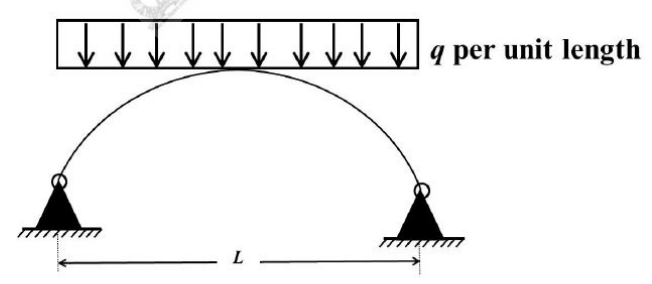
\includegraphics[width=0.5\textwidth]{figures/7.png}
\end{center}
The maximum bending moment in the arch is equal to}{7}

\begin{enumerate}
    \item[(A)] \(\frac{qL^2}{8}\)
    \item[(B)] \(\frac{qL^2}{12}\)
    \item[(C)] zero
    \item[(D)] \(\frac{qL^2}{10}\)
\end{enumerate}

\vspace{0.5cm}

\questiona{Group I lists the type of gain or loss of strength in soils. Group II lists the property or process responsible for the loss or gain of strength in soils.

\begin{tabular}{|l|l|}
\hline
Group I & Group II \\
\hline
P. Regain of strength with time & 1. Boiling \\
Q. Loss of strength due to cyclic loading & 2. Liquefaction \\
R. Loss of strength due to upward seepage & 3. Thixotropy \\
S. Loss of strength due to remolding & 4. Sensitivity \\
\hline
\end{tabular}

The correct match between Group I and Group II is}{8}
\begin{enumerate}
    \item[(A)] P-4, Q-1, R-2, S-3
    \item[(B)] P-3, Q-1, R-2, S-4
    \item[(C)] P-3, Q-2, R-1, S-4
    \item[(D)] P-4, Q-2, R-1, S-3
\end{enumerate}

\vspace{0.5cm}

\questiona{A soil sample is subjected to a hydrostatic pressure, $\sigma$. The Mohr circle for any point in the soil sample would be}{9}
\begin{enumerate}
    \item[(A)] a circle of radius $\sigma$ and center at the origin
    \item[(B)] a circle of radius $\sigma$ and center at a distance $\sigma$ from the origin
    \item[(C)] a point at a distance $\sigma$ from the origin
    \item[(D)] a circle of diameter $\sigma$ and center at the origin
\end{enumerate}

\vspace{0.5cm}

\questiona{A strip footing is resting on the ground surface of a pure clay bed having an undrained cohesion $c_{u}$. The ultimate bearing capacity of the footing is equal to}{10}
\begin{enumerate}
    \item[(A)] $2\pi c_{u}$
    \item[(B)] $\pi c_{u}$
    \item[(C)] $(\pi+1) c_{u}$
    \item[(D)] $(\pi+2) c_{u}$
\end{enumerate}

\vspace{0.5cm}

\questiona{A uniformly distributed line load of 500 kN/m is acting on the ground surface. Based on Boussinesq's theory, the ratio of vertical stress at a depth 2 m to that at 4 m, right below the line of loading, is}{11}
\begin{enumerate}
    \item[(A)] 0.25
    \item[(B)] 0.5
    \item[(C)] 2.0
    \item[(D)] 4.0
\end{enumerate}

\vspace{0.5cm}

\questiona{For a steady incompressible laminar flow between two infinite parallel stationary plates, the shear stress variation is}{12}
\begin{enumerate}
    \item[(A)] linear with zero value at the plates
    \item[(B)] linear with zero value at the center
    \item[(C)] quadratic with zero value at the plates
    \item[(D)] quadratic with zero value at the center
\end{enumerate}

\vspace{0.5cm}

\questiona{The reaction rate involving reactants $A$ and $B$ is given by $-k[A]^{\alpha}[B]^{\beta}$. Which one of the following statements is valid for the reaction to be a first-order reaction?}{13}
\begin{enumerate}
    \item[(A)] $\alpha = 0$ and $\beta = 0$
    \item[(B)] $\alpha = 1$ and $\beta = 0$
    \item[(C)] $\alpha = 1$ and $\beta = 1$
    \item[(D)] $\alpha = 1$ and $\beta = 2$
\end{enumerate}

\vspace{0.5cm}

\questiona{The wastewater from a city, containing a high concentration of biodegradable organics, is being steadily discharged into a flowing river at a location S. If the rate of aeration of the river water is lower than the rate of degradation of the organics, then the dissolved oxygen of the river water}{14}
\begin{enumerate}
    \item[(A)] is lowest at the location S.
    \item[(B)] is lowest at a point upstream of the location S.
    \item[(C)] remains constant all along the length of the river.
    \item[(D)] is lowest at a point downstream of the location S.
\end{enumerate}

\vspace{0.5cm}

\questiona{Which one of the following is NOT present in the acid rain?}{15}
\begin{enumerate}
    \item[(A)] HNO$_3$
    \item[(B)] H$_2$SO$_4$
    \item[(C)] H$_2$CO$_3$
    \item[(D)] CH$_3$COOH
\end{enumerate}

\vspace{0.5cm}

\questiona{A super-elevation $e$ is provided on a circular horizontal curve such that a vehicle can be stopped on the curve without sliding. Assuming a design speed $v$ and maximum coefficient of side friction $f_{max}$, which one of the following criteria should be satisfied?}{16}
\begin{enumerate}
    \item[(A)] $e \leq f_{max}$
    \item[(B)] $e > f_{max}$
    \item[(C)] no limit on $e$ can be set
    \item[(D)] $e = \frac{1 - (f_{max})^2}{f_{max}}$
\end{enumerate}

\vspace{0.5cm}

\questiona{A runway is being constructed in a new airport as per the International Civil Aviation Organization (ICAO) recommendations. The elevation and the airport reference temperature of this airport are 535 m above the mean sea level and 22.65°C, respectively. Consider the effective gradient of runway as 1\%. The length of runway required for a design-aircraft under the standard conditions is 2000 m. Within the framework of applying sequential corrections as per the ICAO recommendations, the length of runway corrected for the temperature is}{17}
\begin{enumerate}
    \item[(A)] 2223 m
    \item[(B)] 2250 m
    \item[(C)] 2500 m
    \item[(D)] 2750 m
\end{enumerate}

\vspace{0.5cm}

\questiona{The accuracy of an Electronic Distance Measuring Instrument (EDMI) is specified as $\pm$(a mm + b ppm). Which one of the following statements is correct?}{18}
\begin{enumerate}
    \item[(A)] Both $a$ and $b$ remain constant, irrespective of the distance being measured.
    \item[(B)] $a$ remains constant and $b$ varies in proportion to the distance being measured.
    \item[(C)] $a$ varies in proportion to the distance being measured and $b$ remains constant.
    \item[(D)] Both $a$ and $b$ vary in proportion to the distance being measured.
\end{enumerate}

\vspace{0.5cm}

\questiona{The number of spectral bands in the Enhanced Thematic Mapper sensor on the remote sensing satellite Landsat-7 is}{19}
\begin{enumerate}
    \item[(A)] 64
    \item[(B)] 10
    \item[(C)] 8
    \item[(D)] 15
\end{enumerate}

\vspace{0.5cm}

\questiona{Consider the following partial differential equation:
\[3 \frac{\partial^2 \phi}{\partial x^2} + B \frac{\partial^2 \phi}{\partial x \partial y} + 3 \frac{\partial^2 \phi}{\partial y^2} + 4 \phi = 0\]
For this equation to be classified as parabolic, the value of $B^2$ must be \_\_\_\_\_.}{20}

\vspace{0.5cm}

\questiona{$\lim_{x \to 0} \left( \frac{\tan x}{x^2 - x} \right)$ is equal to \_\_\_\_\_.}{21}

\vspace{0.5cm}

\questiona{A 3 m thick clay layer is subjected to an initial uniform pore pressure of 145 kPa. The coefficient of consolidation $c_v = 3.0$ mm$^2$/min and $T_{v(90)} = 0.85$. The time (in days, rounded to the nearest integer) required for 90\% consolidation would be \_\_\_\_\_.}{22}
\begin{center}
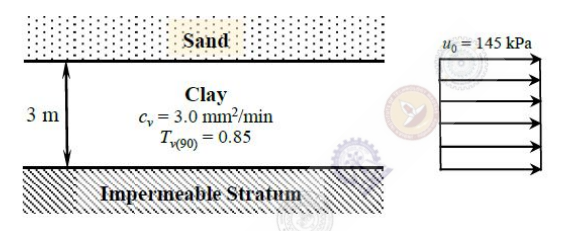
\includegraphics[width=0.5\textwidth]{figures/22.png}
\end{center}

\vspace{0.5cm}

\questiona{A triangular pipe network is shown in the figure with head loss in each pipe given by $h_f = rQ^{1.8}$. The value of $r$ for pipe AB is 1 and for pipe BC is 2. If the discharge supplied at point A (100) is equally divided between pipes AB and AC, the value of $r$ (up to two decimal places) for pipe AC should be \_\_\_\_\_.}{23}
\begin{center}
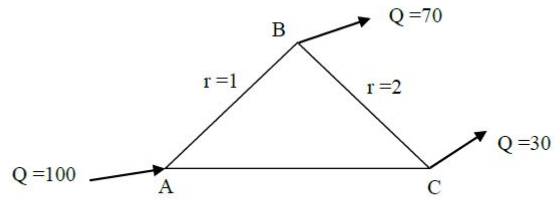
\includegraphics[width=0.5\textwidth]{figures/23.png}
\end{center}

\vspace{0.5cm}

\questiona{The ordinates of a 2-hour unit hydrograph for a catchment are given as:
\begin{tabular}{|c|c|c|c|c|c|}
\hline
Time (h) & 0 & 1 & 2 & 3 & 4 \\
\hline
Ordinate (m$^3$/s) & 0 & 5 & 12 & 25 & 41 \\
\hline
\end{tabular}
The ordinate (in m$^3$/s) of a 4-hour unit hydrograph for this catchment at the time of 3 h would be \_\_\_\_\_.}{24}

\vspace{0.5cm}

\questiona{Vehicles arriving at an intersection from one of the approach roads follow the Poisson distribution. The mean rate of arrival is 900 vehicles per hour. If a gap is defined as the time difference between two successive vehicle arrivals, the probability (up to four decimal places) that the gap is greater than 8 seconds is \_\_\_\_\_.}{25}

\vspace{0.5cm}

\questionb{For the function $f(x) = a + bx$, $0 \leq x \leq 1$, to be a valid probability density function, which one of the following statements is correct?}{26}
\begin{enumerate}
    \item[(A)] $a = 1$, $b = 4$
    \item[(B)] $a = 0.5$, $b = 1$
    \item[(C)] $a = 0$, $b = 1$
    \item[(D)] $a = 1$, $b = -1$
\end{enumerate}

\vspace{0.5cm}

\questionb{The solution of the equation $\frac{dQ}{dt} + Q = 1$ with $Q = 0$ at $t = 0$ is}{27}
\begin{enumerate}
    \item[(A)] $Q(t) = e^{-t} - 1$
    \item[(B)] $Q(t) = 1 + e^{-t}$
    \item[(C)] $Q(t) = 1 - e^{t}$
    \item[(D)] $Q(t) = 1 - e^{-t}$
\end{enumerate}

\vspace{0.5cm}

\questionb{Consider the matrix $\begin{bmatrix} 5 & -1 \\ 4 & 1 \end{bmatrix}$. Which one of the following statements is TRUE for the eigenvalues and eigenvectors of this matrix?}{28}
\begin{enumerate}
    \item[(A)] Eigenvalue 3 has a multiplicity of 2, and only one independent eigenvector exists.
    \item[(B)] Eigenvalue 3 has a multiplicity of 2, and two independent eigenvectors exist.
    \item[(C)] Eigenvalue 3 has a multiplicity of 2, and no independent eigenvector exists.
    \item[(D)] Eigenvalues are 3 and $-3$, and two independent eigenvectors exist.
\end{enumerate}

\vspace{0.5cm}

\questionb{A planar truss tower structure is shown in the figure. 
\begin{center}
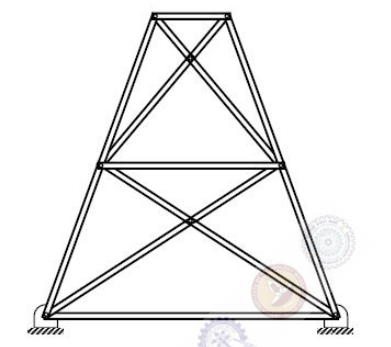
\includegraphics[width=0.5\textwidth]{figures/29.png}
\end{center}
Consider the following statements about the external and internal determinacies of the truss:
\begin{itemize}
    \item[(P)] Externally Determinate
    \item[(Q)] External Static Indeterminacy = 1
    \item[(R)] External Static Indeterminacy = 2
    \item[(S)] Internally Determinate
    \item[(T)] Internal Static Indeterminacy = 1
    \item[(U)] Internal Static Indeterminacy = 2
\end{itemize}
Which one of the following options is correct?}{29}
\begin{enumerate}
    \item[(A)] P-False; Q-True; R-False; S-False; T-False; U-True
    \item[(B)] P-False; Q-True; R-False; S-False; T-True; U-False
    \item[(C)] P-False; Q-False; R-True; S-False; T-False; U-True
    \item[(D)] P-True; Q-True; R-False; S-True; T-False; U-True
\end{enumerate}

\vspace{0.5cm}

\questionb{Group I contains three broad classes of irrigation supply canal outlets. Group II presents hydraulic performance attributes.
\begin{center}
\begin{tabular}{|l|l|}
\hline
Group I & Group II \\
\hline
P. Non-modular outlet & 1. Outlet discharge depends on both supply canal and receiving water course levels \\
Q. Semi-modular outlet & 2. Outlet discharge is fixed and independent of water levels \\
R. Modular outlet & 3. Outlet discharge depends only on supply canal level \\
\hline
\end{tabular}
\end{center}
The correct match of the items in Group I with the items in Group II is}{30}
\begin{enumerate}
    \item[(A)] P - 1; Q - 2; R - 3
    \item[(B)] P - 3; Q - 1; R - 2
    \item[(C)] P - 2; Q - 3; R - 1
    \item[(D)] P - 1; Q - 3; R - 2
\end{enumerate}

\vspace{0.5cm}

\questionb{A 1 m wide rectangular channel has a bed slope of 0.0016 and the Manning's roughness coefficient is 0.04. Uniform flow takes place in the channel at a flow depth of 0.5 m.At a particular section, gradually varies flow (GVF) is observed and the flow depth is measured as 0.6 m. The GVF profile at that section is classified as}{31}
\begin{enumerate}
    \item [(A)] $S_1$
    \item[(B)]$S_2$
    \item[(C)] $M_1$
    \item[(D)] $M_2$ 
\end{enumerate}

\vspace{0.5cm}

\questionb{The following observations are made while testing aggregate for pavement construction:
\begin{itemize}
    \item[i.] Mass of oven-dry aggregate in air = 1000 g
    \item[ii.] Mass of saturated surface-dry aggregate in air = 1025 g
    \item[iii.] Mass of saturated surface-dry aggregate under water = 625 g
\end{itemize}
Based on these observations, the correct statement is}{32}
\begin{enumerate}
    \item[(A)] bulk specific gravity = 2.5 and water absorption = 2.5\%
    \item[(B)] bulk specific gravity = 2.5 and water absorption = 2.4\%
    \item[(C)] apparent specific gravity = 2.5 and water absorption = 2.5\%
    \item[(D)] apparent specific gravity = 2.5 and water absorption = 2.4\%
\end{enumerate}

\vspace{0.5cm}

\questionb{The queue length versus time plot for an approach to a signalized intersection with cycle length of 96 seconds is shown.
\begin{center}
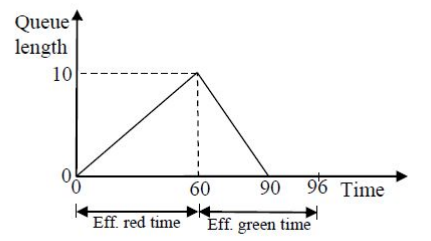
\includegraphics[width=0.5\textwidth]{figures/33.png}
\end{center}
At time $t = 0$, the light has just turned red. The effective green time is 36 seconds, during which vehicles discharge at saturation flow rate $s$. Vehicles arrive at uniform rate $v$ throughout the cycle. Which statement is TRUE?}{33}
\begin{enumerate}
    \item[(A)] $v = 600$ vph, average stopped delay = 30 seconds
    \item[(B)] $s = 1800$ vph, average stopped delay = 28.125 seconds
    \item[(C)] $v = 600$ vph, average stopped delay = 45 seconds
    \item[(D)] $s = 1200$ vph, average stopped delay = 28.125 seconds
\end{enumerate}

\vspace{0.5cm}

\questionb{The radius of a horizontal circular curve on a highway is 120 m. The design speed is 60 km/hour, and the design coefficient of lateral friction is 0.15. The estimated value of superelevation required (if full lateral friction is assumed to develop), and the value of coefficient of friction needed (if no superelevation is provided) will, respectively, be}{34}
\begin{enumerate}
    \item[(A)] $\frac{1}{11.6}$ and 0.10
    \item[(B)] $\frac{1}{10.5}$ and 0.37
    \item[(C)] $\frac{1}{11.6}$ and 0.24
    \item[(D)] $\frac{1}{12.9}$ and 0.24
\end{enumerate}

\vspace{0.5cm}

\questionb{The observed bearings of a traverse are given below:
\begin{center}
\begin{tabular}{|l|l|l|l|}
\hline
Line & Bearing & Line & Bearing \\
\hline
PQ & $46^\circ15'$ & QP & $226^\circ15'$ \\
QR & $108^\circ15'$ & RQ & $286^\circ15'$ \\
RS & $201^\circ30'$ & SR & $20^\circ30'$ \\
ST & $321^\circ45'$ & TS & $141^\circ45'$ \\
\hline
\end{tabular}
\end{center}
The station(s) most likely to be affected by local attraction is/are}{35}
\begin{enumerate}
    \item[(A)] Only R
    \item[(B)] Only S
    \item[(C)] R and S
    \item[(D)] P and Q
\end{enumerate}

\vspace{0.5cm}

\questionb{The laboratory tests on a soil sample yields the following results: natural moisture content = 18\%, liquid limit = 60\%, plastic limit = 25\%, percentage of clay sized fraction = 25\%. The liquidity index and activity (as per the expression proposed by Skempton) of the soil, respectively, are}{36}
\begin{enumerate}
    \item[(A)] -0.2 and 1.4
    \item[(B)] 0.2 and 1.4
    \item[(C)] -1.2 and 0.714
    \item[(D)] 1.2 and 0.714
\end{enumerate}

\vspace{0.5cm}

\questionb{Consider the equation $\frac{du}{dt} = 3t^2 + 1$ with $u = 0$ at $t = 0$. This is numerically solved by using the forward Euler method with a step size, $\Delta t = 2$. The absolute error in the solution at the end of the first time step is \_\_\_\_\_.}{37}

\vspace{0.5cm}

\questionb{A pre-tensioned rectangular concrete beam 150 mm wide and 300 mm depth is prestressed with three straight tendons, each having a cross-sectional area of 50 mm$^2$, to an initial stress of 1200 N/mm$^2$. The tendons are located at 100 mm from the soffit of the beam. If the modular ratio is 6, the loss of prestressing force (in kN, up to one decimal place) due to the elastic deformation of concrete only is \_\_\_\_\_.}{38}

\vspace{0.5cm}

\questionb{Consider the stepped bar made with a linear elastic material and subjected to an axial load of 1 kN, as shown in the figure. 
\begin{center}
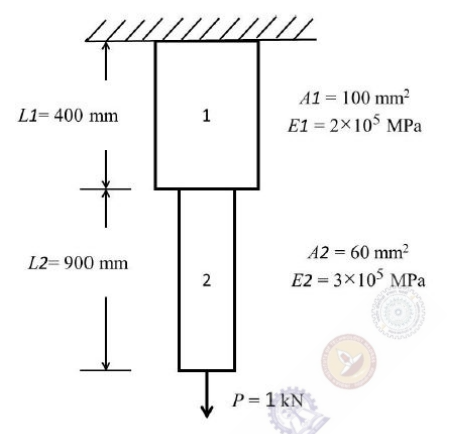
\includegraphics[width=0.5\textwidth]{figures/39.png}
\end{center}
Segments 1 and 2 have cross-sectional area of 100 mm$^2$ and 60 mm$^2$, Young's modulus of $2 \times 10^5$ MPa and $3 \times 10^5$ MPa, and length of 400 mm and 900 mm, respectively. The strain energy (in N-mm, up to one decimal place) in the bar due to the axial load is \_\_\_\_\_.}{39}

\vspace{0.5cm}

\questionb{The value of M in the beam ABC shown in the figure is such that the joint B does not rotate.
\begin{center}
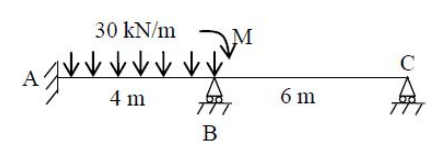
\includegraphics[width=0.5\textwidth]{figures/40.png}
\end{center}
The value of support reaction (in kN) at B should be equal to \_\_\_\_\_.}{40}

\vspace{0.5cm}

\questionb{Consider the beam ABCD shown in the figure with AB = BC = 4 m and CD = 10 m. 
\begin{center}
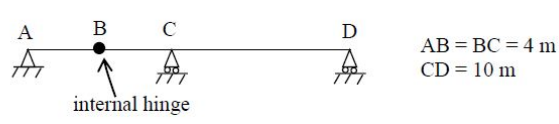
\includegraphics[width=0.5\textwidth]{figures/41.png}
\end{center}
For a moving concentrated load of 50 kN on the beam, the magnitude of the maximum bending moment (in kN-m) obtained at the support C will be equal to \_\_\_\_\_.}{41}

\vspace{0.5cm}

\questionb{Consider two axially loaded columns, namely, 1 and 2, made of a linear elastic material with Young's modulus $2 \times 10^5$ MPa, square cross-section with side 10 mm, and length 1 m. For Column 1, one end is fixed and the other end is free. For Column 2, one end is fixed and the other end is pinned. Based on the Euler's theory, the ratio (up to one decimal place) of the buckling load of Column 2 to the buckling load of Column 1 is \_\_\_\_\_.}{42}

\vspace{0.5cm}

\questionb{A column is subjected to a load through a bracket as shown in the figure.
\begin{center}
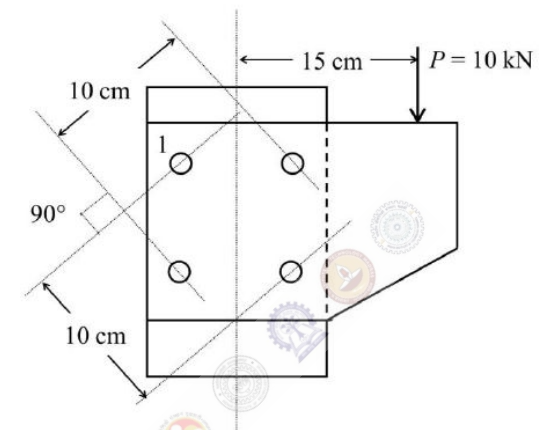
\includegraphics[width=0.5\textwidth]{figures/43.png}
\end{center}
The resultant force (in kN, up to one decimal place) in the bolt 1 is \_\_\_\_\_.}{43}

\vspace{0.5cm}

\questionb{A particle of mass 2 kg is travelling at a velocity of 1.5 m/s. A force $f(t) = 3t^2$ (in N) is applied to it in the direction of motion for a duration of 2 seconds. The velocity (in m/s, up to one decimal place) of the particle immediately after the removal of the force is \_\_\_\_\_.}{44}

\vspace{0.5cm}

\questionb{The activity details of a project are given below:
\begin{center}
\begin{tabular}{|l|l|l|}
\hline
Activity & Depends on & Duration (days) \\
\hline
P & -- & 6 \\
Q & P & 15 \\
R & Q, T & 12 \\
S & R & 16 \\
T & P & 10 \\
U & Q, T & 14 \\
V & U & 16 \\
\hline
\end{tabular}
\end{center}
The estimated minimum time (in days) for the completion of the project will be \_\_\_\_\_.}{45}

\vspace{0.5cm}

\questionb{It is proposed to drive H-piles up to a depth of 7 m at a construction site. The average surface area of the H-pile is 3 m$^2$ per meter length. The soil at the site is homogeneous sand, having an effective friction angle of 32°. The ground water table (GWT) is at a depth of 2 m below the ground surface. The unit weights of the soil above and below the GWT are 16 kN/m$^3$ and 19 kN/m$^3$, respectively. Assume the earth pressure coefficient, $K = 1.0$, and the angle of wall friction, $\delta = 23^\circ$. The total axial frictional resistance (in kN, up to one decimal place) mobilized on the pile against the driving is \_\_\_\_\_.}{46}

\vspace{0.5cm}

\questionb{The infinite sand slope shown in the figure is on the verge of sliding failure. The ground water table coincides with the ground surface. Unit weight of water $\gamma_w = 9.81$ kN/m$^3$, $\gamma_{sat} = 21$ kN/m$^3$.
\begin{center}
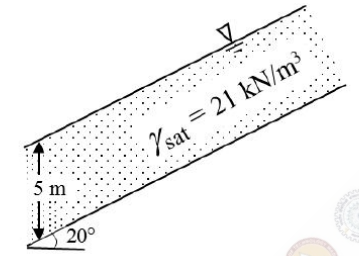
\includegraphics[width=0.5\textwidth]{figures/47.png}
\end{center}
The value of the effective angle of internal friction (in degrees, up to one decimal place) of the sand is \_\_\_\_\_.}{47}

\vspace{0.5cm}

\questionb{A sluice gate used to control the flow in a horizontal channel of unit width is shown in the figure. 
\begin{center}
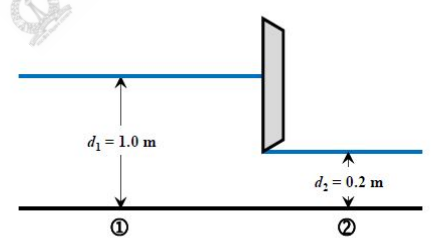
\includegraphics[width=0.5\textwidth]{figures/48.png}
\end{center}
It is observed that the depth of flow is 1.0 m upstream of the gate, while the depth is 0.2 m downstream of the gate. Assuming a smooth flow transition across the sluice gate without any energy loss, and the acceleration due to gravity as 10 m/s$^2$, the discharge (in m$^3$/s, up to two decimal places) passing under the sluice gate is \_\_\_\_\_.}{48}

\vspace{0.5cm}

\questionb{Water flows through a 90° bend in a horizontal plane as depicted in the figure.
\begin{center}
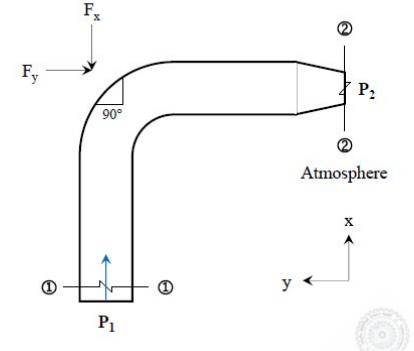
\includegraphics[width=0.5\textwidth]{figures/49.png}
\end{center}
A pressure of 140 kPa is measured at Section 1-1. The inlet diameter marked at Section 1-1 is $\frac{27}{\sqrt{\pi}}$ cm, while the nozzle diameter marked at Section 2-2 is $\frac{14}{\sqrt{\pi}}$ cm. Assume: (i) Acceleration due to gravity = 10 m/s$^2$, (ii) Weights of both the bent pipe segment and water are negligible, (iii) Friction across the bend is negligible. The magnitude of the force (in kN, up to two decimal places) that would be required to hold the pipe section is \_\_\_\_\_.}{49}

\vspace{0.5cm}

\questionb{A consolidated undrained (CU) triaxial compression test is conducted on a normally consolidated clay at a confining pressure of 100 kPa. The deviator stress at failure is 80 kPa, and the pore-water pressure measured at failure is 50 kPa. The effective angle of internal friction (in degrees, up to one decimal place) of the soil is \_\_\_\_\_.}{50}

\vspace{0.5cm}

\questionb{An effective rainfall of 2-hour duration produced a flood hydrograph peak of 200 m$^3$/s. The flood hydrograph has a base flow of 20 m$^3$/s. If the spatial average rainfall in the watershed for the duration of storm is 2 cm and the average loss rate is 0.4 cm/hour, the peak of 2-hour unit hydrograph (in m$^3$/s-cm, up to one decimal place) is \_\_\_\_\_.}{51}

\vspace{0.5cm}

\questionb{The equivalent sound power level (in dB) of the four sources with the noise levels of 60 dB, 69 dB, 70 dB and 79 dB is \_\_\_\_\_.}{52}

\vspace{0.5cm}

\questionb{The spherical grit particles, having a radius of 0.01 mm and specific gravity of 3.0, need to be separated in a settling chamber. Given: $g = 9.81$ m/s$^2$, density of the liquid = 1000 kg/m$^3$, kinematic viscosity of the liquid = $10^{-6}$ m$^2$/s. Assuming laminar conditions, the settling velocity (in mm/s, up to one decimal place) is \_\_\_\_\_.}{53}

\vspace{0.5cm}

\questionb{Two wastewater streams A and B, having an identical ultimate BOD are getting mixed to form the stream C. The temperature of the stream A is 20°C and the temperature of the stream C is 10°C. Given: the 5-day BOD of the stream A measured at 20°C = 50 mg/l, BOD rate constant (base 10) at 20°C = 0.115 per day, temperature coefficient = 1.135. The 5-day BOD (in mg/l, up to one decimal place) of the stream C, calculated at 10°C, is \_\_\_\_\_.}{54}

\vspace{0.5cm}

\questionb{The wastewater having an organic concentration of 54 mg/l is flowing at a steady rate of 0.8 m$^3$/day through a detention tank of dimensions 2 m × 4 m × 2 m. If the contents of the tank are well mixed and the decay constant is 0.1 per day, the outlet concentration (in mg/l, up to one decimal place) is \_\_\_\_\_.}{55}

\vspace{0.5cm}

\vspace{5cm}
\begin{center}
\textbf{END OF THE QUESTION PAPER}
\rule{\textwidth}{0.5pt} 
\end{center}

\end{document}